% ==================================================================================
% W-STTran++ Method — Detailed Technical Report
% Target Venue: NeurIPS
% ==================================================================================
\documentclass{article}

% Uncomment if neurips_2026.sty is available
% \usepackage[preprint]{neurips_2026}
% Fallback to standard margins if neurips is unavailable:
\usepackage[margin=1in]{geometry}

\usepackage[utf8]{inputenc}
\usepackage{amsmath,amssymb,amsfonts}
\usepackage{graphicx}
\usepackage{booktabs}
\usepackage{algorithm}
\usepackage{algpseudocode}
\usepackage{bm}
\usepackage{xcolor}
\usepackage{tikz}
\usetikzlibrary{arrows.meta,positioning,shapes.geometric,fit,calc,backgrounds}

\newcommand{\mR}{\mathbb{R}}
\newcommand{\op}[1]{\operatorname{#1}}
\newcommand{\mat}[1]{\bm{#1}}

\title{W-STTran++: Enhanced World Scene Graph Generation without Explicit Tracking}
\author{Anonymous Authors}

\begin{document}

\maketitle

% ====================================================================================
\section{Introduction}
\label{sec:intro}
% ====================================================================================

The W-STTran++ architecture is an enhanced adaptation of the STTran method for the World Scene Graph Generation (WorldSGG) task. While the base W-STTran model relies entirely on passive memory and 3D geometric spatial attention, W-STTran++ introduces several critical features for world-aware reasoning: (1) an \emph{ObjectSpatialEncoder} that explicitly models camera-relative object positions; (2) an \emph{ObjectMotionEncoder} that captures 3D object dynamics; and (3) a \emph{TemporalEdgeAttention} module that reasons about relationships across frames. 

Notably, W-STTran++ does \emph{not} include explicit temporal object tracking (e.g., TemporalObjectEncoder), serving as an ablation to measure the impact of camera and motion features when an object's visual representation is maintained solely by a zero-order memory buffer. W-STTran++ utilizes a FasterRCNN-ResNet50 backbone.

% ====================================================================================
\section{Pipeline Overview}
\label{sec:pipeline}
% ====================================================================================

Figure~\ref{fig:pipeline_wsttran_pp} illustrates the complete pipeline. Object appearances are buffered, then enriched with 3D structural, camera-relative, and motion features. Following intra-frame inter-object reasoning, a temporal edge attention mechanism resolves relationship predictions across time.

\begin{figure}[h]
\centering
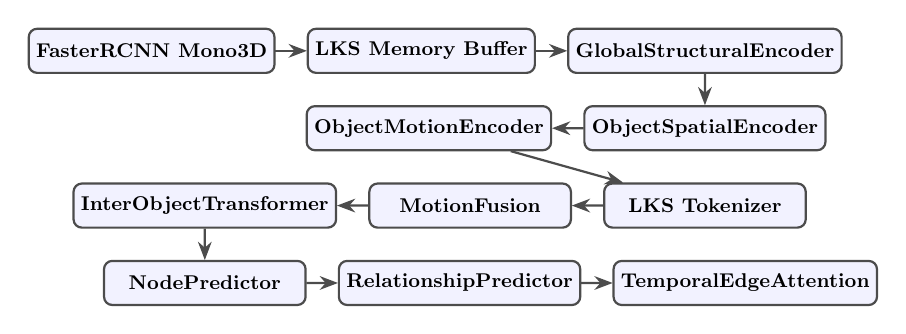
\begin{tikzpicture}[
  scale=0.8, transform shape, >=Stealth,
  block/.style={draw=black!70, rounded corners=3pt, line width=0.8pt, fill=blue!5, minimum width=3.2cm, minimum height=0.7cm, font=\small\bfseries, align=center},
  arrow/.style={->, thick, black!70}
]

\node[block] (mono) {FasterRCNN Mono3D};
\node[block, right=0.5cm of mono] (buffer) {LKS Memory Buffer};
\node[block, right=0.5cm of buffer] (gse) {GlobalStructuralEncoder};
\node[block, below=0.5cm of gse] (ose) {ObjectSpatialEncoder};
\node[block, left=0.5cm of ose] (ome) {ObjectMotionEncoder};
\node[block, below=0.5cm of ose] (tok) {LKS Tokenizer};
\node[block, left=0.5cm of tok] (fuse) {MotionFusion};
\node[block, left=0.5cm of fuse] (iot) {InterObjectTransformer};
\node[block, below=0.5cm of iot] (np) {NodePredictor};
\node[block, right=0.5cm of np] (rp) {RelationshipPredictor};
\node[block, right=0.5cm of rp] (tea) {TemporalEdgeAttention};

\draw[arrow] (mono) -- (buffer);
\draw[arrow] (buffer) -- (gse);
\draw[arrow] (gse) -- (ose);
\draw[arrow] (ose) -- (ome);
\draw[arrow] (ome) -- (tok);
\draw[arrow] (tok) -- (fuse);
\draw[arrow] (fuse) -- (iot);
\draw[arrow] (iot) -- (np);
\draw[arrow] (np) -- (rp);
\draw[arrow] (rp) -- (tea);

\end{tikzpicture}
\caption{The W-STTran++ pipeline. It extends the minimal W-STTran baseline by incorporating camera-relative spatial features, 3D object motion, and temporal relationship attention.}
\label{fig:pipeline_wsttran_pp}
\end{figure}

% ====================================================================================
\section{LKS Memory Buffer}
\label{sec:lks}
% ====================================================================================

The LKS (Last Known State) Memory Buffer provides non-differentiable visual persistence. For an object $n$ at frame $t$, the buffered feature $\mat{m}_n^{(t)}$ is defined by:
\begin{equation}
    \mat{m}_n^{(t)} = \begin{cases}
        \mat{f}_n^{(t)} & \text{if object $n$ is visible at $t$}, \\
        \mat{f}_n^{(\tau^*)} & \text{where } \tau^* = \arg\min_{\tau:\text{vis}(n,\tau)} |t - \tau|, \\
        \bm{0} & \text{if object $n$ is never seen}.
    \end{cases}
    \label{eq:lks_buffer}
\end{equation}
The staleness $\Delta_n^{(t)} = |t - \tau^*|$ is also computed and clamped to a sentinel value (1000) for never-seen objects.

% ====================================================================================
\section{GlobalStructuralEncoder}
\label{sec:gse}
% ====================================================================================

The \emph{GlobalStructuralEncoder} grounds features in 3D world geometry using 8-corner oriented bounding boxes (OBBs) $\mat{C}_n \in \mR^{8 \times 3}$. It computes the centered local corners:
\begin{align}
    \bar{\mat{c}}_n &= \frac{1}{8}\sum_{i=1}^{8}\mat{c}_{n,i} \in \mR^{3}, \label{eq:center} \\
    \tilde{\mat{c}}_{n,i} &= \mat{c}_{n,i} - \bar{\mat{c}}_n \in \mR^{3}, \quad i=1,\dots,8. \label{eq:local}
\end{align}
The local corners and absolute center are passed through an MLP to generate per-object structural tokens $\mat{g}_n$:
\begin{equation}
    \mat{g}_n = \op{MLP}_{\text{obj}}\bigl([\op{flatten}(\tilde{\mat{c}}_{n,i}) \;\|\; \bar{\mat{c}}_n]\bigr) \in \mR^{d_{\text{struct}}}.
    \label{eq:gse_obj}
\end{equation}

% ====================================================================================
\section{ObjectSpatialEncoder}
\label{sec:ose}
% ====================================================================================

Unlike standard VidSGG, WorldSGG involves moving cameras. The \emph{ObjectSpatialEncoder} (formerly CameraPoseEncoder) computes camera-relative features for each object.

Given the camera extrinsic matrix $\mat{T} = [\mat{R}\,|\,\boldsymbol{\tau}]$, we encode the global camera token:
\begin{equation}
    \mat{c}_{\text{cam}} = \op{MLP}_{\text{cam}}\bigl([\op{6D}(\mat{R}) \;\|\; \boldsymbol{\tau}]\bigr) \in \mR^{d_{\text{camera}}},
    \label{eq:cam_global}
\end{equation}
where $\op{6D}(\mat{R})$ is the continuous 6D rotation representation. For each object $n$, camera-relative features are computed:
\begin{align}
    \mat{d}_n &= \bar{\mat{c}}_n - \boldsymbol{\tau}, \quad \text{(direction)} \label{eq:cam_dir} \\
    \alpha_n &= \hat{\mat{d}}_n \cdot (-\mat{R}_{:,2}), \quad \text{(view alignment)} \label{eq:view_align} \\
    \beta_n^{\sin},\,\beta_n^{\cos} &= \hat{\mat{d}}_n \cdot \mat{R}_{:,0},\; \alpha_n. \quad \text{(azimuth)} \label{eq:azimuth}
\end{align}
These are projected to a per-object spatial representation:
\begin{equation}
    \mat{c}_n = \op{MLP}\bigl([\log\|\mat{d}_n\|,\;\alpha_n,\;\beta_n^{\sin},\;\beta_n^{\cos}]\bigr) \in \mR^{d_{\text{camera}}}.
    \label{eq:cam_per_obj}
\end{equation}

% ====================================================================================
\section{ObjectMotionEncoder}
\label{sec:ome}
% ====================================================================================

The \emph{ObjectMotionEncoder} captures 3D dynamics directly from world-frame OBB centers:
\begin{align}
    \mat{v}_n^{(t)} &= \bar{\mat{c}}_n^{(t)} - \bar{\mat{c}}_n^{(t-1)}, \quad \text{(velocity)} \label{eq:velocity} \\
    \mat{a}_n^{(t)} &= \mat{v}_n^{(t)} - \mat{v}_n^{(t-1)}. \quad \text{(acceleration)} \label{eq:accel}
\end{align}
A camera-relative velocity $\mat{v}_n^{\text{cam}} = \mat{R}^{\!\top}\mat{v}_n$ provides parallax-aware motion. The combined 11-dimensional feature vector $[\mat{v}_n,\,\mat{a}_n,\,\|\mat{v}_n\|,\,\mat{v}_n^{\text{cam}},\,\|\mat{v}_n^{\text{cam}}\|]$ is projected via MLP to produce motion features $\mat{\mu}_n^{(t)} \in \mR^{d_{\text{motion}}}$.

% ====================================================================================
\section{LKS Tokenizer and Motion Fusion}
\label{sec:tokenizer_fusion}
% ====================================================================================

The Tokenizer concatenates geometry, buffer, spatial, and staleness features:
\begin{equation}
    \mat{x}_n^{(t)} = \op{FusionProj}\bigl([\mat{g}_n^{(t)} \;\|\; \mat{m}_n^{(t)} \;\|\; \mat{c}_n^{(t)} \;\|\; \log(\Delta_n^{(t)} + 1)]\bigr) \in \mR^{d_{\text{model}}}.
    \label{eq:tokenizer}
\end{equation}
The resulting token is then fused with the object motion features via an additive projection with LayerNorm and GELU:
\begin{equation}
    \hat{\mat{x}}_n^{(t)} = \op{LayerNorm}\bigl(\op{Linear}([\mat{x}_n^{(t)} \;\|\; \mat{\mu}_n^{(t)}])\bigr) \in \mR^{d_{\text{model}}}.
    \label{eq:fusion}
\end{equation}

% ====================================================================================
\section{InterObjectTransformer and Node Predictor}
\label{sec:iot_np}
% ====================================================================================

The \emph{InterObjectTransformer} performs intra-frame spatial reasoning globally across objects. It utilizes continuous pairwise 3D spatial positional encodings $\mat{S}^{(t)}$:
\begin{equation}
    \mat{H}^{(t)} = \op{TransformerEncoder}\bigl(\hat{\mat{X}}^{(t)} + \mat{S}^{(t)},\; \text{mask}=\overline{\mat{v}}^{(t)}\bigr) \in \mR^{N \times d_{\text{model}}}.
    \label{eq:iot}
\end{equation}
The \emph{Node Predictor} then classifies the refined object representations using a two-layer MLP to output logits $\hat{\mat{Y}}^{\text{obj}}$.

% ====================================================================================
\section{Relationship Predictor and Temporal Edge Attention}
\label{sec:tea}
% ====================================================================================

Initial relationship tokens $\mat{r}_{po}$ are formed from subject, object, union visual features, and semantic embeddings, followed by intra-frame relationship self-attention.

W-STTran++ introduces \emph{TemporalEdgeAttention} for cross-frame reasoning. For a unique object pair $(p, o)$, relationship tokens across all frames are collected, augmented with a learned temporal positional embedding $\mat{e}_\tau$, and processed by a temporal transformer:
\begin{equation}
    \tilde{\mat{r}}_{po}^{(t)} = \op{TemporalEncoder}\bigl(\{{\mat{r}}_{po}^{(\tau)} + \mat{e}_{\tau}\}_{\tau \in \mathcal{T}_{po}}\bigr).
    \label{eq:tea}
\end{equation}
The temporally-refined tokens are passed to independent MLP heads to predict final attention, spatial, and contacting logits.

% ====================================================================================
\section{Loss Function}
\label{sec:loss}
% ====================================================================================

The loss function partitions pair predictions into visible and unseen groups. Unseen pair pseudo-labels (provided by VLMs) are smoothed and weighted by $\lambda_{\text{vlm}}$:
\begin{equation}
    \mathcal{L}_{\text{W-STTran++}} = \sum_{r \in \{\text{att, spa, con}\}} \bigl(\mathcal{L}_{r}^{\text{vis}} + \mathcal{L}_{r}^{\text{unseen}}\bigr) + \mathcal{L}_{\text{node}}.
    \label{eq:loss}
\end{equation}

% ====================================================================================
\section{Algorithm: Forward Pass}
\label{sec:algorithm}
% ====================================================================================

\begin{algorithm}[h]
\caption{W-STTran++ Forward Pass}
\begin{algorithmic}[1]
\Require $\mat{f}_{\text{all}}$ (visual), $\mat{C}_{\text{all}}$ (OBBs), $\mat{T}_{\text{all}}$ (camera)
\Ensure $\hat{\mat{y}}_{\text{att}}, \hat{\mat{y}}_{\text{spa}}, \hat{\mat{y}}_{\text{con}}$
\State $(\mat{m}_{\text{all}}, \bm{\Delta}_{\text{all}}) \gets \text{LKS\_Buffer}(\mat{f}_{\text{all}})$
\State $\mat{G}_{\text{all}} \gets \text{GlobalStructuralEncoder}(\mat{C}_{\text{all}})$
\State $\mat{c}_{\text{all}} \gets \text{ObjectSpatialEncoder}(\mat{T}_{\text{all}}, \mat{C}_{\text{all}})$
\State $\mat{\mu}_{\text{all}} \gets \text{ObjectMotionEncoder}(\mat{C}_{\text{all}}, \mat{T}_{\text{all}})$
\State $\mat{X} \gets \text{Tokenizer}(\mat{G}_{\text{all}}, \mat{m}_{\text{all}}, \mat{c}_{\text{all}}, \log \bm{\Delta}_{\text{all}})$
\State $\hat{\mat{X}} \gets \text{MotionFusion}(\mat{X}, \mat{\mu}_{\text{all}})$
\State $\mat{H} \gets \text{InterObjectTransformer}(\hat{\mat{X}})$
\State $\hat{\mat{Y}}^{\text{obj}} \gets \text{NodePredictor}(\mat{H})$
\State $\mat{R} \gets \text{RelationshipFormationAndSelfAttention}(\mat{H}, \hat{\mat{Y}}^{\text{obj}})$
\State $\tilde{\mat{R}} \gets \text{TemporalEdgeAttention}(\mat{R})$
\State $(\hat{\mat{y}}_{\text{att}}, \hat{\mat{y}}_{\text{spa}}, \hat{\mat{y}}_{\text{con}}) \gets \text{PredictionHeads}(\tilde{\mat{R}})$
\State \Return $\hat{\mat{y}}_{\text{att}}, \hat{\mat{y}}_{\text{spa}}, \hat{\mat{y}}_{\text{con}}$
\end{algorithmic}
\end{algorithm}

\end{document}
